\pdfoutput=1
\documentclass[
  12pt,
  oneside,
  a4paper,
  chapter=TITLE,
  section=TITLE,
  brazil
]{abntex2}

% ===============================
% PACOTES BÁSICOS
% ===============================
\usepackage[utf8]{inputenc}
\usepackage[T1]{fontenc}
\usepackage{lmodern}
\usepackage{indentfirst}
\usepackage{graphicx}
\usepackage{float}
\usepackage{amsmath,amssymb,amsfonts}
\usepackage{microtype}
\usepackage[hidelinks]{hyperref}
\usepackage{setspace}
\usepackage{mathrsfs}

\graphicspath{{figuras/}}

% ===============================
% BIBLIOGRAFIA (ABNT)
% ===============================
\usepackage[alf]{abntex2cite}

% ===============================
% DADOS DO TRABALHO
% ===============================
\autor{Thales Machado Fernandes}

\titulo{%
NOVOS MATERIAIS BIDIMENSIONAIS OBTIDOS PELA ENGENHARIA DE DEFEITOS PARA
ARMAZENAMENTO E REAÇÕES DE EVOLUÇÃO DE HIDROGÊNIO
}

\local{Santo André}
\data{2026}
\orientador{Prof.\ Pedro Alves da Silva Autreto}

\instituicao{%
  Universidade Federal do ABC
  \par
  Bacharelado Interdisciplinar em Ciência e Tecnologia
}

\tipotrabalho{Trabalho de Conclusão do PRH}

\preambulo{%
Trabalho apresentado como requisito final para o PRH.
}

% ===============================
% DOCUMENTO
% ===============================
\begin{document}

\selectlanguage{brazil}
\frenchspacing
\OnehalfSpacing

% ===============================
% ELEMENTOS PRÉ-TEXTUAIS
% ===============================

\begin{capa}
\centering

{\ABNTEXchapterfont\bfseries\Large
UNIVERSIDADE FEDERAL DO ABC\par}

\vspace{2cm}


\includegraphics[width=0.35\textwidth]{logo_faculdade.png}

\vspace{2cm}

{\ABNTEXchapterfont\bfseries\large
Thales Machado Fernandes\par}

\vspace{1cm}

{\ABNTEXchapterfont\bfseries\large
NOVOS MATERIAIS BIDIMENSIONAIS OBTIDOS PELA ENGENHARIA DE DEFEITOS PARA
ARMAZENAMENTO E REAÇÕES DE EVOLUÇÃO DE HIDROGÊNIO\par}

\vfill

{\large
Santo André\par}
{\large
2026\par}

\end{capa}

\imprimirfolhaderosto

\begin{epigrafe}
\vspace*{\fill}
\begin{flushright}
\textit{"Se eu não quiser ser vaporizado em uma explosão nuclear, simplesmente terei que me tornar nuclear eu mesmo... Eu sou atômico."}\\
--- Cid Kagenou
\end{flushright}
\end{epigrafe}

\begin{resumo}

A crescente demanda por fontes de energia sustentáveis tem impulsionado o desenvolvimento de tecnologias voltadas à produção de hidrogênio, especialmente por meio de processos eletroquímicos livres de emissão de carbono. No entanto, a eficiência desses processos é limitada pela cinética da reação de evolução de hidrogênio (HER), que depende fortemente do uso de catalisadores. Embora a platina seja o material mais eficiente para essa finalidade, seu alto custo e baixa abundância restringem sua aplicação em larga escala, motivando a busca por materiais alternativos.

Neste trabalho, foi investigado o potencial catalítico do grafeno modificado por defeitos estruturais do tipo Stone-Wales, utilizando métodos de teoria do funcional da densidade (DFT) e sua aproximação DFTB. Foram construídas diferentes configurações de defeitos, incluindo padrões de linhas e estruturas do tipo shuriken, com o objetivo de analisar como a organização e interação entre defeitos influenciam a atividade catalítica do material. A eficiência foi avaliada por meio da energia livre de adsorção de hidrogênio ($\Delta G$), parâmetro amplamente utilizado como descritor da atividade na HER.

Os resultados indicam que a presença e a organização de defeitos de Stone-Wales promovem uma melhora significativa na atividade catalítica do grafeno, especialmente em regiões de interação entre defeitos, onde foram observados valores de $\Delta G$ mais próximos do ideal. Além disso, foi identificado que a formação de múltiplos defeitos induz curvatura na estrutura, gerando uma assimetria entre os dois lados da folha e influenciando diretamente os valores de $\Delta G$. Foi observada uma forte correlação entre a curvatura local e a diferença de energia de adsorção, indicando que a geometria do material desempenha um papel fundamental na catálise.

A comparação entre os métodos DFT e DFTB revelou boa concordância qualitativa nas tendências observadas, embora com diferenças quantitativas relevantes, sugerindo que o DFTB pode ser utilizado como ferramenta eficiente para análise exploratória de sistemas maiores, com menor custo computacional.

Dessa forma, os resultados obtidos demonstram que a engenharia de defeitos em materiais de carbono, em particular no grafeno, constitui uma estratégia promissora para o desenvolvimento de catalisadores eficientes e de baixo custo para a produção de hidrogênio.

\textbf{Palavras-chave}: HER. DFT. Grafeno.
\end{resumo}

\begin{resumo}[Abstract]
The increasing demand for sustainable energy sources has driven the development of technologies aimed at hydrogen production, particularly through electrochemical processes with low carbon emissions. However, the efficiency of these processes is limited by the kinetics of the hydrogen evolution reaction (HER), which strongly depends on the use of efficient catalysts. Although platinum is recognized as the most effective catalyst for HER, its high cost and limited availability hinder its large-scale application, motivating the search for alternative materials.

In this work, the catalytic potential of graphene modified by Stone–Wales structural defects was investigated using density functional theory (DFT) and its approximation, DFTB. Different defect configurations were constructed, including line patterns and shuriken-like structures, in order to analyze how the arrangement and interaction of defects influence the catalytic activity of the material. The performance was evaluated through the hydrogen adsorption free energy ($\Delta G$), a widely used descriptor for HER activity.

The results indicate that the presence and organization of Stone–Wales defects significantly enhance the catalytic activity of graphene, particularly in regions where defects interact, where $\Delta G$ values closer to the ideal were observed. Furthermore, the formation of multiple defects induces curvature in the structure, leading to asymmetry between the two sides of the graphene sheet and directly affecting the adsorption energy. A strong correlation between local curvature and the difference in $\Delta G$ was identified, highlighting the crucial role of geometry in catalytic performance.

The comparison between DFT and DFTB methods shows good qualitative agreement in the observed trends, despite noticeable quantitative differences, suggesting that DFTB can be effectively used for exploratory studies of larger systems with reduced computational cost.

Overall, the results demonstrate that defect engineering in carbon-based materials, particularly graphene, is a promising strategy for the development of efficient and low-cost catalysts for hydrogen production.

\textbf{Keywords}: HER. DFT. Graphene.
\end{resumo}

\tableofcontents
\listoffigures
\listoftables

% ===============================
% PARTE TEXTUAL
% ===============================
\textual

\chapter{Introdução}

Texto da introdução.

Exemplo de citação \cite{einstein1905}.


\chapter{Fundamentacao Teórica}

\section{Postulados da Mecânica Quântica}

A física quântica surgiu em meio a descoberta de que tanto ondas eletromagnéticas \
quanto partículas, poderiam apresentar comportamentos ondulatóricos e corpusculares a depender do experimento. \
Além disso, a formulaçao clássica baseada nas leis de newton falhava na descrição de tais sistemas, o que \
levou a um grande esforço da comunidade científica por um formalismo mais acertivo.

A descrição inicial mais completa da mecânica quântica aborda uma descrição probabilística dos sistemas em pequena escala. \
Essa descrição é muito motivada por fatos experimetais e abordagens teóricas antecedentes, \
tais como a dualidade onda-partícula, a ideia de onda de matéria de de Broglie, e a quantização \
da energia de Planck. O sucesso empírico dessa teoria faz com que seja amplamente utilizada \
em pesquisas atuais, em especial na física da matéria condensada.

Os aspectos mais fundamentais da mecânica quântica podem ser resumidos em seus postulados.

\subsection{Primeiro Postulado}

Assim como na mecânica clássica os sistemas possuem um conjunto de variáveis que definem o estado de um sistema, \
como por exemplo a posição e o momento, na mecânica quântica assumimos que nosso sistema também pode assumir \
um conjunto de estados representados como vetores no espaço de Hilbert denotados por $|k\rangle$. Contudo, diferente da mecânica clássica, \
um sistema quântico pode estar em uma superposição de estados físicos. Isso é descrito matemáticamente como uma \
combinação linear no caso de estados discretos,
\begin{equation}
    |\psi\rangle=\sum_k c_k |k\rangle,
\end{equation}
como por exemplo o spin do eletron, ou, quando lidamos com estados contínuos, como a posição de uma partícula, \
a superposição se da por uma integral sobre todos os estados,
\begin{equation}
    |\psi \rangle = \int dk ~c(k) |k \rangle.
\end{equation}

\subsection{Segundo Postulado}

De fato, o estado de um sistema quantico ser uma combinação linear de seus possíveis estados \
não tem um significado físico evidente. Portanto, essa interpretação é postulada de modo que possamos compreender \
o que o formalismo matemático representa na realidade. O segundo postulado da mecânica quântica afirma que se os estados são ortonormais, isso é, 
\begin{equation}
    \langle i | j \rangle = \delta_{ij}
\end{equation}
no caso discreto, e
\begin{equation}
    \langle \xi | \xi' \rangle = \delta(\xi-\xi')
\end{equation}
no caso contínuo, a probabilidade \
de se encontrar um sistema quântico no estado $|k\rangle$ é $|\langle k | \psi \rangle|^2$, os coeficientes da combinação linear, \
de modo que a probabilidade de achar o sistem em qualquer estado é
\begin{equation}
    \langle \psi | \psi \rangle = (\sum_k c_k^* \langle k |)(\sum_k c_k |k\rangle) = \sum_k |c_k|^2 = \sum_k |\langle k | \psi \rangle|^2 = 1
\end{equation}
ou
\begin{equation}
    \langle \psi | \psi \rangle = (\int dk ~c^*(k)\langle k |)(\int dk' ~c(k')|k'\rangle)=\int\int dk dk' ~c^*(k)c(k')\delta(k-k') = \int dk ~|c(k)|^2 = 1,
\end{equation}
como deve ser.

\subsection{Terceiro Postulado}

Uma medida de uma variável física como a posição, momento ou energia, em um sistema quântico, é representado por uma operação no estado do sistema. \
Essa operação é mediada por um objeto chamado operador, $\hat A$, que é linear e atua sobre o ket, de modo que os únicos valores possíveis de serem obtidos \
pela medição, $a_k$, são os que satisfazem a equação
\begin{equation}
    \hat A |\psi_k \rangle = a_k |\psi_k \rangle.
\end{equation}
Os estados $|\psi_k\rangle$ são conhecidos como autoestados de $\hat A$, enquanto que $a_k$ são seus autovalores.

\subsection{Quarto Postulado}

Os operadores $\hat x$ e $\hat p$ tem sua atuação conhecida na base de posições, 
\begin{equation}
    \hat x |\psi\rangle =  \int dx ~\psi(x) \hat x|x \rangle = \int dx ~\psi(x) x|x \rangle
\end{equation}
\begin{equation}
    \langle x|\hat x |\psi\rangle =  x \psi(x).
\end{equation}
Além disso, pode-se obter apartir dessa relação que
\begin{equation}
    \langle x|\hat p |\psi\rangle =  -i\hbar \frac{\partial}{\partial x} \psi(x).
\end{equation}
O quarto postulado afirma que se conhecemos uma função clássica $f(x,p)$ que depende da posição e do momento, e que queremos medi-la, podemos obter \
o seu respectivo operador na mecânica quântica promovendo a posição e o momento aos operadores de posição e moemnto,
\begin{equation}
    x, ~p \to \hat x, ~\hat p
\end{equation}
\begin{equation}
    f(x,p) \to f(\hat x,\hat p)
\end{equation}

\subsection{Quinto Postulado}

Se soubermos o estado de um sistema quântico em um dado instante, e queremos saber qual será seu estado \
em um período de tempo depois, recorremos ao quinto postulado que afirma que a evolução temporal de um sistema quântico \
é descrita pela equação de Schrodinger,
\begin{equation}
i\hbar \frac{\partial}{\partial t}|\psi\rangle = \hat H |\psi\rangle
\end{equation}
em que $\hat H$ é o operador Hamiltoniano,
\begin{equation}
    \hat H = \frac{\hat p^2}{2m} + \hat V,
\end{equation}
cujos autovalores são as possíveis energias do sistema.

\section{Estados Estacionários}

Em muitas situações importantes na física, o a energia potêncial não depende do tempo, \
ou simplesmente tratamos como se nao dependesse. Nesse caso especial, podemos reescrever \
equação de Schrodinger de forma mais conveniente.

Partindo da equação de Schrodinger e projetando na base de posição, temos que
\begin{equation}
    i\hbar \langle x | \frac{\partial}{\partial t}|\Psi\rangle = \langle x |(\frac{\hat p^2}{2m} + \hat V) |\Psi\rangle,
\end{equation}
logo
\begin{equation}
    i\hbar \frac{\partial}{\partial t}\Psi(x,t) = (- \frac{\hbar^2}{2m}\frac{\partial^2}{\partial x^2} + V(x)) \Psi(x,t)
\end{equation}
Assumindo uma solução do tipo $\Psi(x,t)=\psi(x)\phi(t)$, é possível separar em duas equações
\begin{equation}
\frac{i\hbar}{\phi(t)} \frac{\partial}{\partial t}\phi(t) = \frac{1}{\psi(x)}(- \frac{\hbar^2}{2m}\frac{\partial^2}{\partial x^2} + V(x)) \psi(x)=E.
\end{equation}
A equação para $\phi(t)$ pode ser resolvida por integração, 
\begin{equation}
    \phi(t) = e^{-i\frac{E}{\hbar}}
\end{equation}
enquanto que a equação para $\psi(x)$,
\begin{equation}
    (- \frac{\hbar^2}{2m}\frac{\partial^2}{\partial x^2} + V(x)) \psi(x) = E \psi(x),
\end{equation}
depende do potêncial, e é conhecida como equação de Schrodinger independente do tempo. \
Ainda de maneira mais geral podemos escrever essa equação como
\begin{equation}
    (- \frac{\hbar^2 \hat p^2}{2m} + V(\hat x)) |\psi\rangle = E |\psi\rangle,
\end{equation}
com $|\Psi(t)\rangle = e^{-i\frac{E}{\hbar}} |\psi\rangle$. \
Esse tipo de equação é chamado de solução estacionária, e possui algumas características importantes.




\chapter{Metodologia}

Texto da met.

Exemplo de citação \cite{einstein1905}.


\chapter{Resultados e Discussão}

\section{Estruturas de Linhas de Defeitos}

Os resultados referentes as simulações das estruturas com padrões de linhas demonstram que os defeitos de Stone-Wales afetam de maneira positiva a eficiência da estrutura na catálise de hidrogênio.\
As figuras \ref{line1} e \ref{line2}, exibem uma melhora do comportamento catalítico nos sítios localizados na região central dos defeitos, e, em especial, em regiões de união entre os defeitos.

\begin{figure}[H]
    \centering
    
\includegraphics[width=0.9\textwidth]{/home/geedai/Desktop/tcc/figuras/lines.jpg}
    \caption{Estruturas com defeitos de padrões de linhas, organizada por espessura da linha no eixo vertical, e distância entre linhas no eixo horizontal. A variação da energia livre de Gibbs é representada pelo mapa de cores.}
    \label{line1}
\end{figure}

\begin{figure}[H]
    \centering
    
\includegraphics[width=0.9\textwidth]{/home/geedai/Desktop/tcc/figuras/linesbottom.jpg}
    \caption{Estruturas com defeitos de padrões de linhas, organizada por espessura da linha no eixo vertical, e distância entre linhas no eixo horizontal. A variação da energia livre de Gibbs é representada pelo mapa de cores.}
    \label{line2}
\end{figure}

Além da mudança clara do $\Delta G$ em relação a estrutura pristina do grafeno, é notável a diferença entre os dois lados da folha de grafeno modificada. A adição de um único defeito mantém a simetria entre os dois lados da folha, mas\
a união entre dois defeitos cria um efeito de rugosidade, como apresentado na figura \ref{buckling} que cria uma diferença no $\Delta G$ em cada lado da mesma estrutura.

\begin{figure}[H]
    \centering
    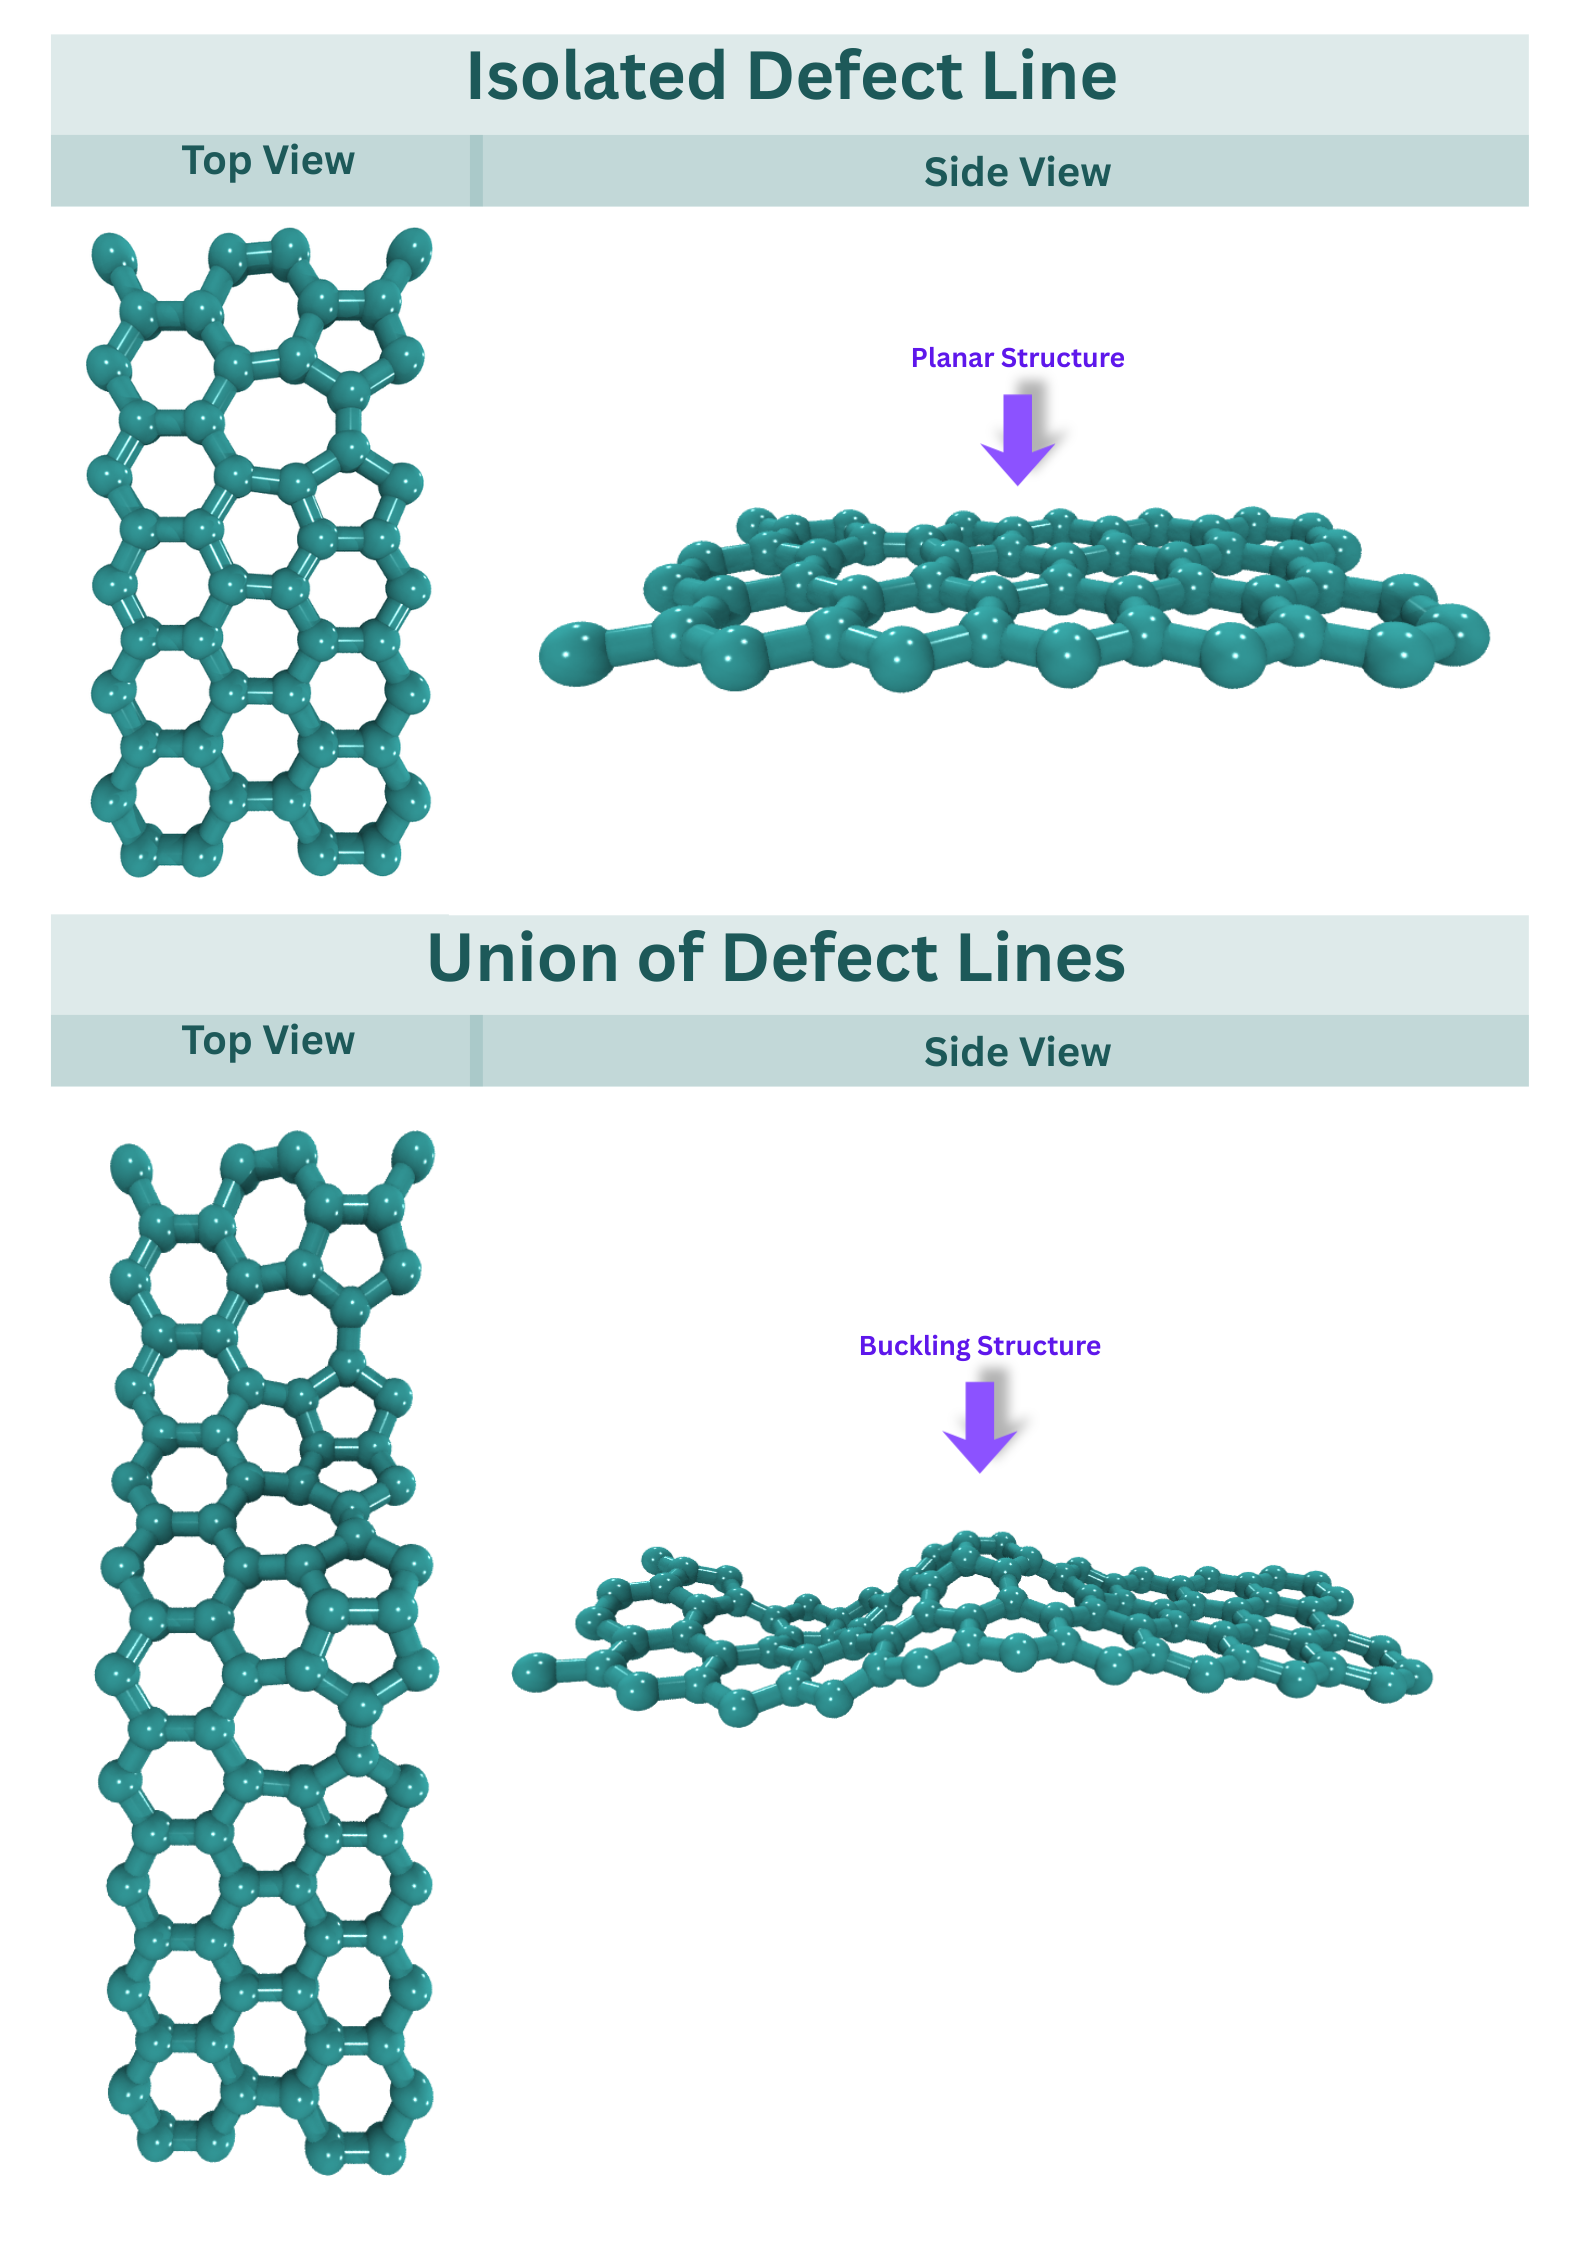
\includegraphics[width=0.9\textwidth]{figuras/Buckling.png}
    \caption{Acima estrutura com uma linha de defeito isolada, e abaixo uma estrutura com união de linhas de defeito.}
    \label{buckling}
\end{figure}

\section{Estruturas de Shuriken}

As estruturas do tipo shuriken-3 e 4 apresentaram redução no valor da energia livre de Gibbs em relação ao grafeno pristino em certos átomos localizados nos aneis dos defeitos de Stone-Wales, formando alguns sítios próprios para a catálise.\
Já o shuriken-6 apresentou uma intensa mudança do $\Delta G$, chegando a valores negativos, e muitos sítios com $\Delta G$ proximos de zero.

Todas as estruturas do tipo shuriken apresentaram efeitos de curvatura em sua superfície que criam as diferenças do $\Delta G$ em cada lado, como apresentado na figura \ref{sks}.
\begin{figure}[H]
    \centering
    
\includegraphics[width=0.9\textwidth]{/home/geedai/Desktop/tcc/figuras/shurikens_dg.png}
    \caption{Estruturas do tipo shuriken com mapa de cor do $\Delta G$ em cada lado da superfície.}
    \label{sks}
\end{figure}

\section{Analise da Curvatura}

Foi observado que a adição de defeitos de Stone-Wales isolados na estrutura do grafeno mantém a superfície plana e portanto simétrica em relação ao eixo z. Por outro lado, a uniao de defeitos gera rugosidade na superfície, criando uma diferença de energia livre de adsorção de hidrogênio em cada lado.\
Dessa forma, faz sentido verificar como a diferença de $\Delta G$ em cada lado é afetada pela curvatura local da superfície.

A relação entre a diferença de $\Delta G$ e a curvatura é exibida na figura \ref{curva1} e \ref{curva2}, apresentando uma grande correlação linear entre esses dois fatores. 

\begin{figure}[H]
    \centering
    
\includegraphics[width=0.9\textwidth]{/home/geedai/Desktop/tcc/figuras/curvature_lines.png}
    \caption{Diferença de $\Delta G$ em cada lado da superfície para cada sítio pela curvatura local no sítio para estruturas de linha.}
    \label{curva1}
\end{figure}

\begin{figure}[H]
    \centering
    
\includegraphics[width=0.9\textwidth]{/home/geedai/Desktop/tcc/figuras/curvature_shuriken.png}
    \caption{Diferença de $\Delta G$ em cada lado da superfície para cada sítio pela curvatura local no sítio para estruturas de shuriken.}
    \label{curva2}
\end{figure}

Os coeficientes angulares das retas ajustadas são A = 4.065 ± 0.144 para estruturas de linhas e A = 3.655 ± 0.319 para estruturas shuriken.


\section{Comparação Entre DFTB e DFT}

A comparação entre os o método do DFT e o DFTB é apresentada na figura \ref{dftb_dft}, em que cada ponto é o valor do $\Delta G$ de um sítio em um dos lados da superfície das estruturas de linha e shuriken. A linha reta se refere aos valores em que os dois métodos concordam, enquanto que valores longe da linha apresentam discrepância entre os métodos.

É evidente que alguns pontos apresentam um grande distânciamento da reta identidade. Contudo, a grande maioria dos pontos seguem a mesma tendência da reta, mas com uma certa defasagem em relação ao eixo vertical.\
Isso sugere que os métodos concordam entre sí quanto ao comportamento do sistema, mas discordam dos valores com um erro quadrático médio (RMSE) de 0.4 eV.

\begin{figure}[H]
    \centering
    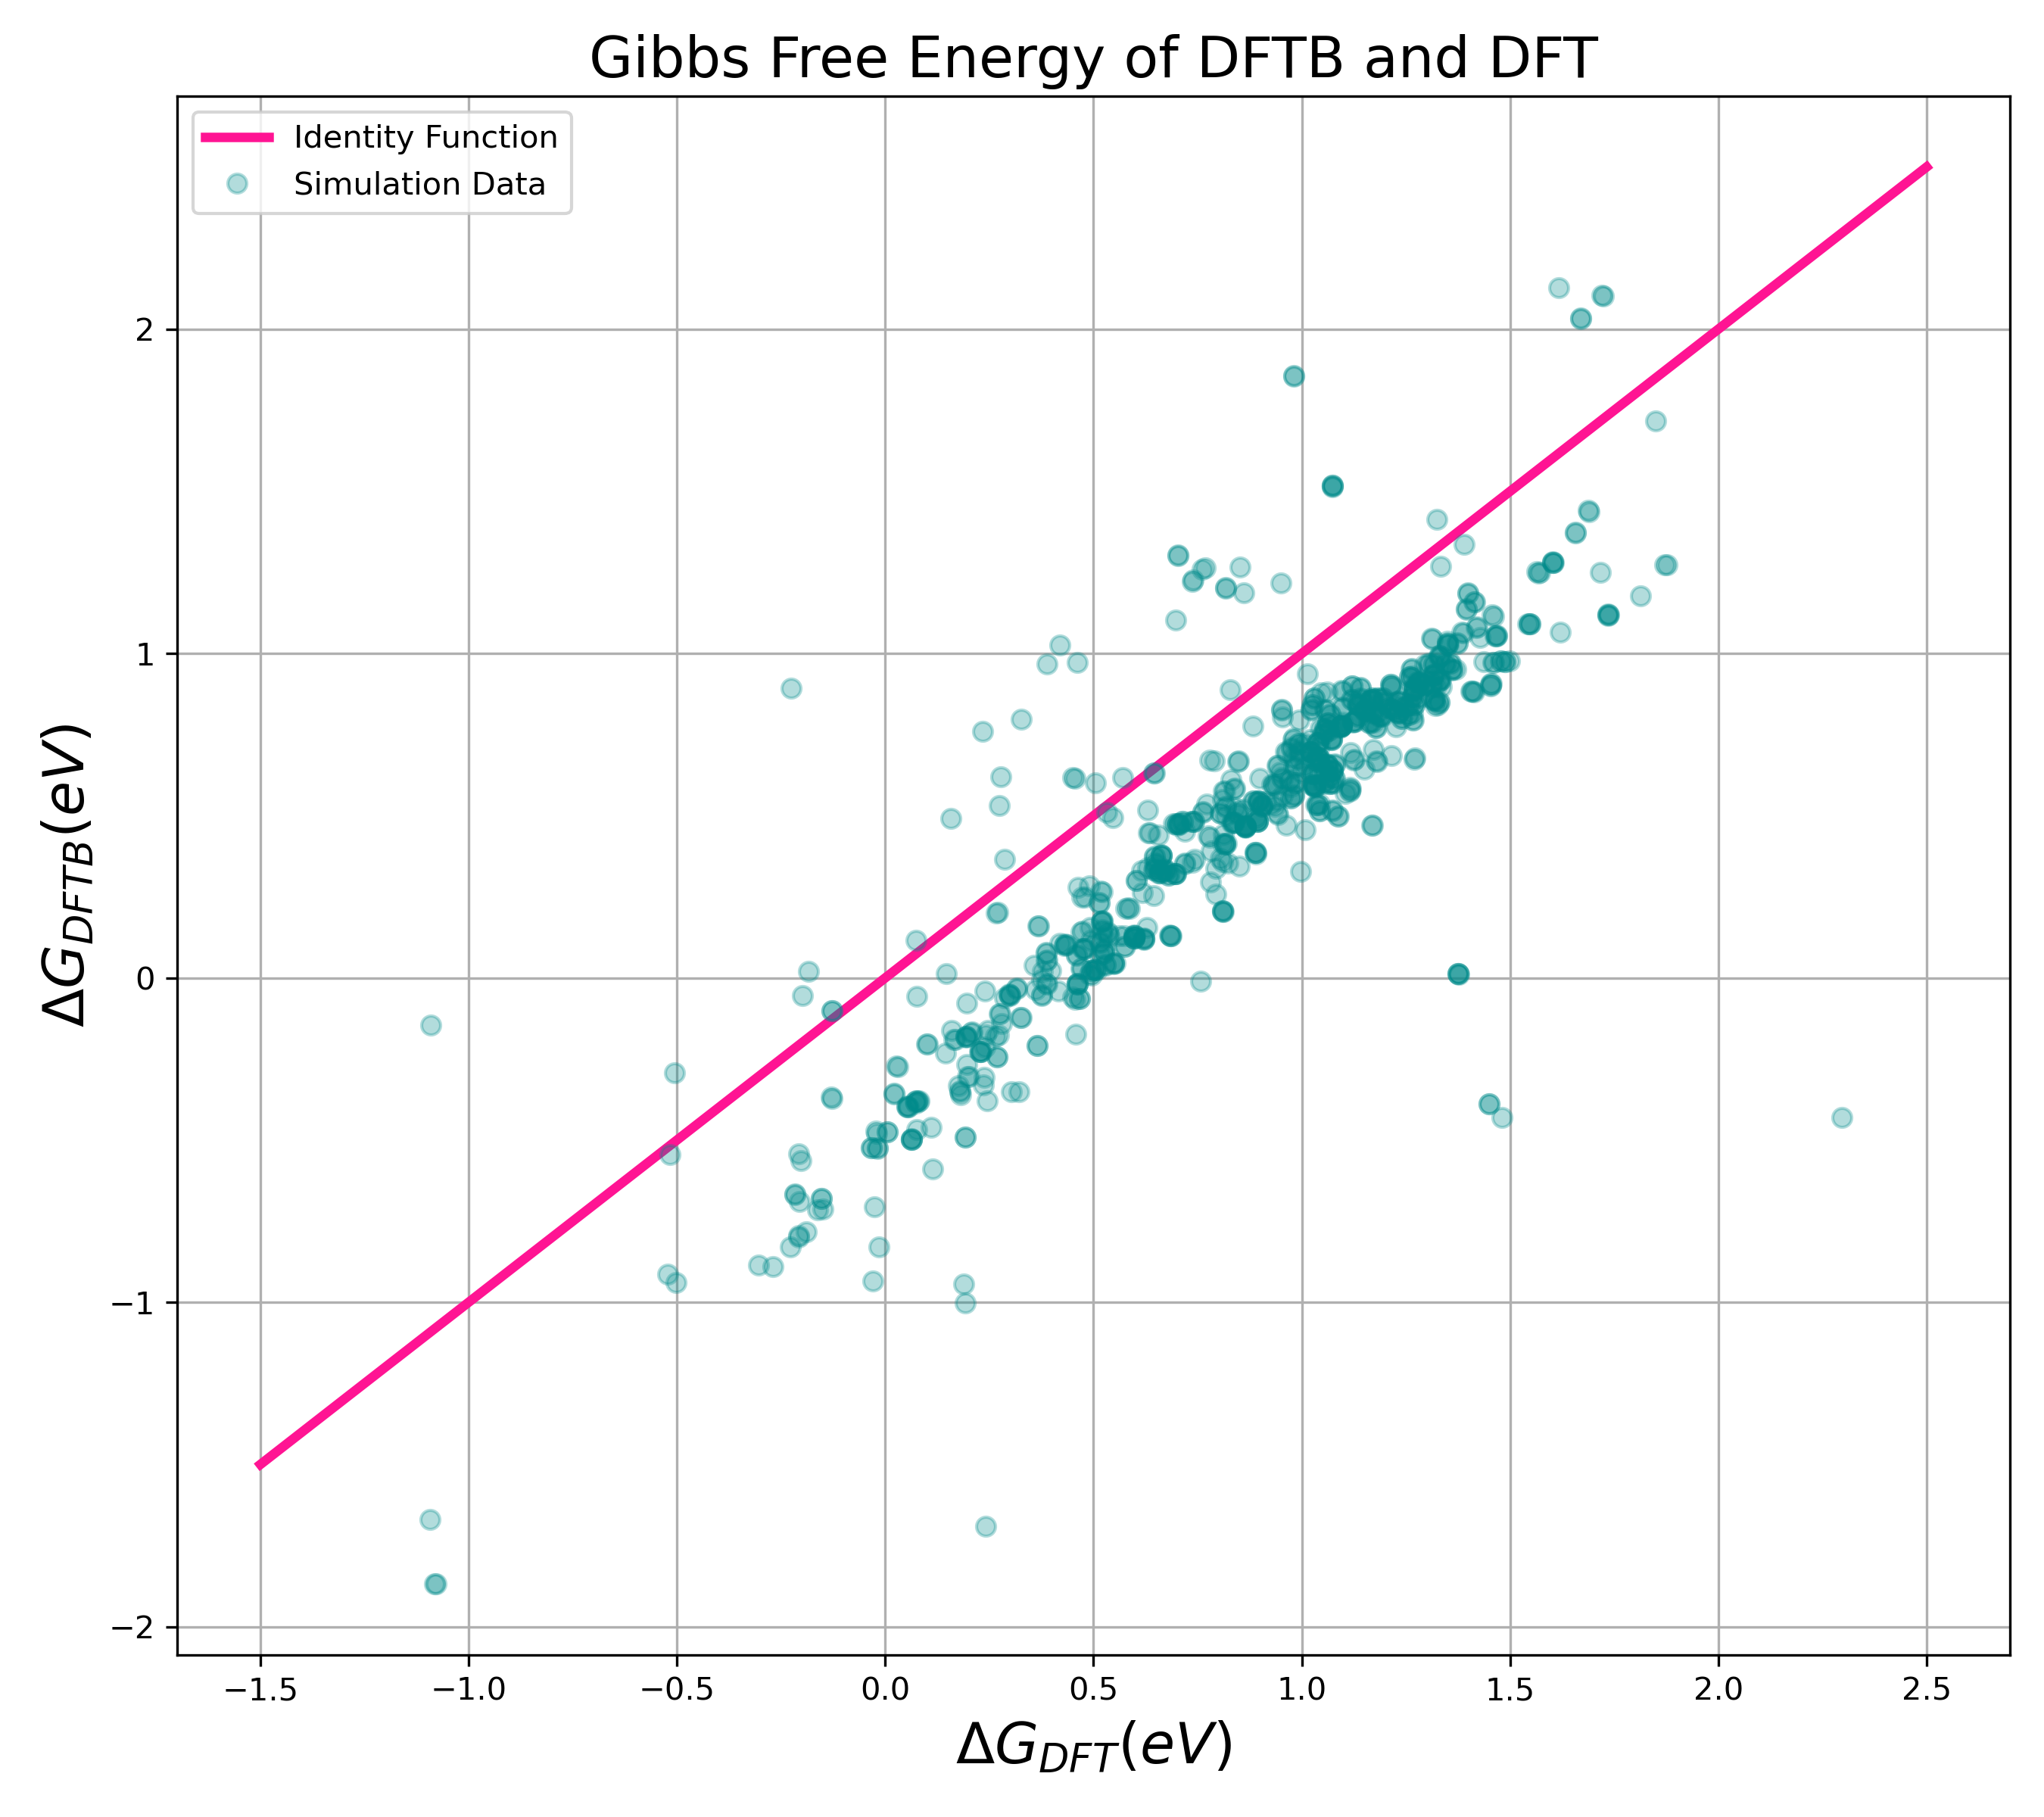
\includegraphics[width=0.9\textwidth]{figuras/dftb_dft.png}
    \caption{Valores de $\Delta G$ para os sítios das estruturas de linha e shuriken utilizando os métodos de DFTB (eixo y) e DFT (eixo x). A linha rosa é a reta identidade.}
    \label{dftb_dft}
\end{figure}

Como a relação entre o DFT e o DFTB é aparentemente linear, pode-se realizar uma correção desse tipo ajustando uma reta no gráfico. Isso é apresentado na figura \ref{dftb_fit},\
onde a reta é $\Delta G_{DFT} = 0.767 \Delta G_{DFTB} + 0.469$ eV. Contudo, o RMSE para o ajuste é de $0.243$, fazendo com que os valores calculados utilizando o DFTB possuem um desvio muito grande em relação ao tamanho da faixa ideal de $\Delta G$.

\begin{figure}[H]
    \centering
    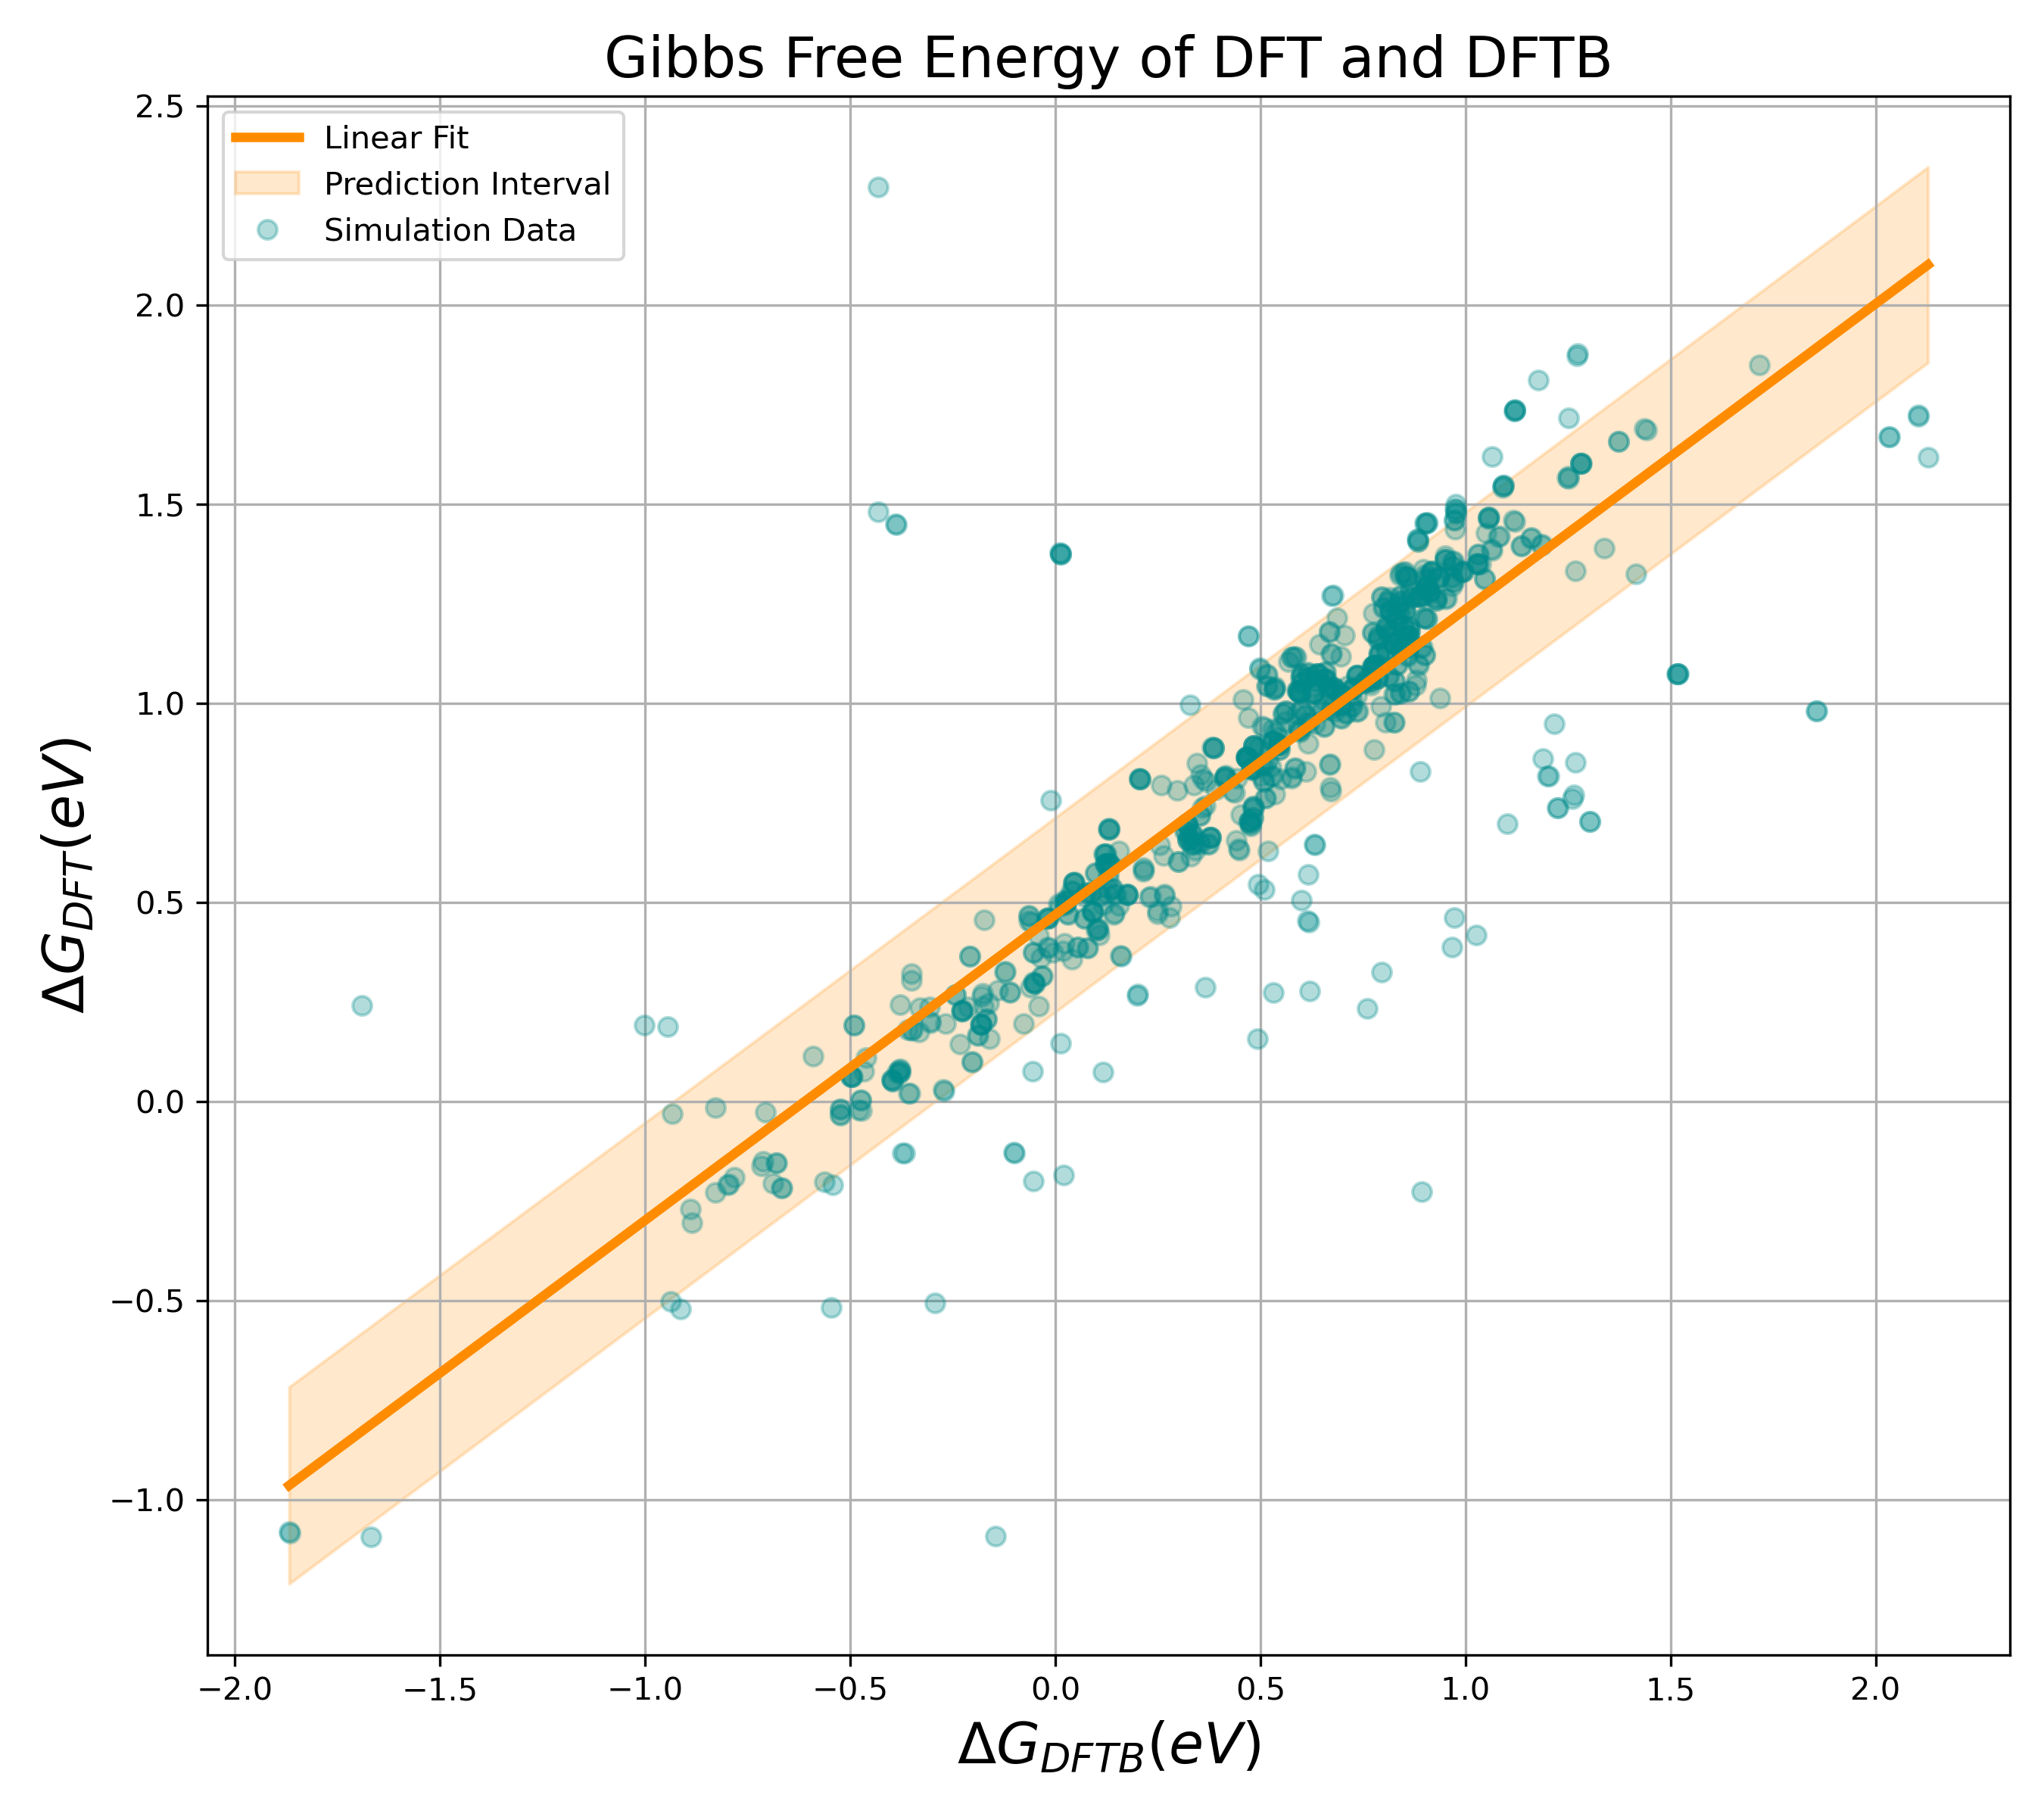
\includegraphics[width=0.9\textwidth]{dftb_dft_fit.png}
    \caption{Valores de $\Delta G$ para os sítios das estruturas de linha e shuriken utilizando os métodos de DFTB (eixo x) e DFT (eixo y). A linha laranja é um ajuste linear, e o sombreamento laranja é a região de incerteza.}
    \label{dftb_fit}
\end{figure}


\include{capitulos/cap5_conclusao}

% ===============================
% REFERÊNCIAS
% ===============================
\bibliography{referencias}

\end{document}
